\documentclass{article}
% \documentclass{beamer}
% \usetheme{Madrid}

%------------------------------
% used for href/url
\usepackage{hyperref}


% used for math fomulas
\usepackage{amsmath}

% used for pictures
\usepackage{graphicx}
\usepackage{subcaption}
\usepackage{float}

% used for codes
\usepackage{listings}
\lstset{
  basicstyle=\ttfamily\footnotesize, % Set your code to be drawn with a monospaced font
  breaklines=true, % Enables line breaking
  frame=single % Adds a frame around the code
}

% used for Graph
\usepackage{adigraph}

% used for Bayesian Network
\usepackage{tikz}
\usetikzlibrary{bayesnet}

%------------------------------
% TODO 
\tolerance=10000
\emergencystretch=\maxdimen
\hyphenpenalty=10000
\hbadness=10000


\usepackage{silence}
\WarningFilter{latex}{Overfull \hbox}

%------------------------------



\title{MK's Notes for CIVL-4530 Geometric Design}
\date{2024-03-04}
\author{Michael Chen}

\begin{document}
  % \pagenumbering{gobble}
  % \maketitle
  % \newpage
  % \pagenumbering{arabic}
  \setcounter{section}{1}


  % todo ----------------------------------------
  % \tableofcontents
  % \newpage


  % ----------------------------------------
  \section{Design Control and Criteria}
  \subsection{Objectives}
  \begin{enumerate}
    \item Design Vehicles, Driver and Traffic Characteristics
    \item 13 AASHTO criteria
    \item AASHTO administered, federal-wide
    \item State-DOT administered - Green Book
    \item local goverment administered - ordinance or code
  \end{enumerate}

  \subsection{Design vehicles}
  \begin{enumerate}
    \item Design Vehicle\\ 
    Its weight, dimensions, and operating characteristics will be used to establish the geometric standards of the highway.
    \item design vehicle P: passenger car
    \begin{enumerate}
      \item Geometry - length 19ft (5+11+3), width 7ft
      \item Minimum turning path - outline 25.4ft, front wheel 23.8ft, CTR 21ft, min 14.4ft 
    \end{enumerate}
    \item WB-50 - length 55ft, width 8.5ft, height 13.5ft
  \end{enumerate}

  ASSHTO guideline - Selection of design vehicle \ref{fig:image-design-vehicles}
  \begin{figure}[!ht]
    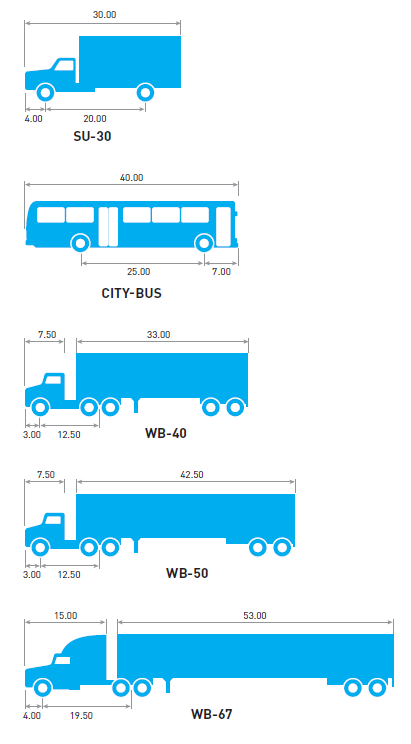
\includegraphics[width=0.7\linewidth]{design-vehicles.png}
    \caption{Design Vehicles}
    \label{fig:image-design-vehicles}
  \end{figure}
  \begin{enumerate}
    \item parking lot - passenger car
    \item intersection of local area - SU-30, 30ft
    \item intersection of state highway and city street - City transit buses, 40ft
    \item intersections of highways; low-volume county roads with ADT < 400 - City bus (40ft, 84 passengers) or conventional bus(36ft, 64 passengers)
    \item freeway ramp; arterial crossroads; intersections of state highways; with high volume of traffic - WB-40 to WB-62
  \end{enumerate}

  \subsection{Older Driver Deficiencies}
  \begin{enumerate}
    \item Slower information processing
    \item Slower reaction times
    \item Slower decision making
    \item Visual deterioration
    \item Hearing deterioration
    \item Decline in ability to judge time, speed, and distance
    \item Limited depth perception
    \item Limited physical mobility
    \item Side effects from prescription drugs
  \end{enumerate}

  \subsection{LOS and ADT}
  acceptable LOS / level of "congestion" \ref*{fig:image-LOS} \\

  \begin{tabular}{|c|c|c|c|c|}
    Roadway & urban & rural level & rural rolling & rural mountainous\\
    \hline
    Freeway & C/D   & B & B & C\\
    Arterial & C/D  & B & B & C\\
    Collector & D   & C & C & D\\
    Local & D       & D & D & D\\
  \end{tabular}
  \begin{figure}[h!]
    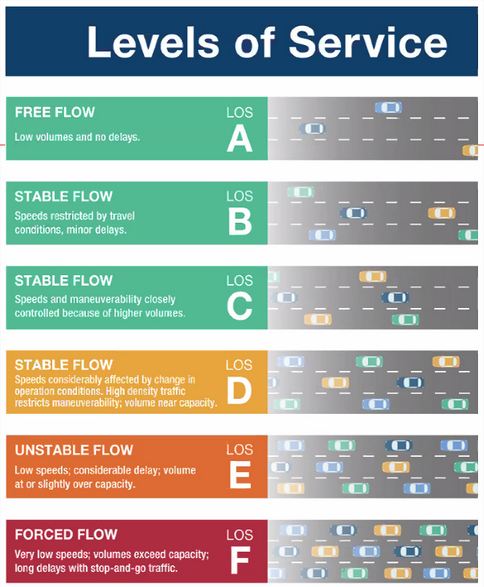
\includegraphics[width=\linewidth]{LOS.png}
    \caption{Level of Service}
    \label{fig:image-LOS}
  \end{figure}

  \subsection{13 AASHTO Criteria}
  \begin{enumerate}
      \item design speed
      \item lane width
      \item shoulder width
      \item bridge width
      \item structural capacity
      \item 
      \item horizontal alignment
      \item vertical alignment
      \item cross slope
      \item grades
      \item superelevation
      \item horizontal clearance
      \item vertical clearance
  \end{enumerate}

  \subsection{speed}
  \begin{enumerate}
    \item running speed - the speed of an individual vehicle
    \item design speed - AASHTO: max safe speed
    \item operation speed - the 85th percentile of observed speed in free flow conditions
    \item safty of over speed - $\Delta$V: [0, 5] low; [5, 15] medium; [15, infinit] high
  \end{enumerate}

  minimum design speed for \textbf{rural} roadways vs vehicle per day(VPD)
  \begin{tabular}{|c|c|c|c|}
    \hline
    rural terrain & 0-400 & 400-2000 & over 2000 \\
    \hline
    level         & 40    & 50       & 60 \\
    rolling       & 30    & 40       & 50 \\
    mountainous   & 20    & 30       & 40 \\
  \end{tabular}

  \subsection{lane width for urban and rural (1-2ft wider than urban)}
  \begin{tabular}{|l|l|l|}
    Types & urban & rural \\
    \hline
    Freeway and Interstates: & 12ft, & 12ft\\
    Ramp: & 12-30ft & 12-30ft \\ 
    Arterial: & 11-12ft, & 10-12ft \\
    Collections: & 10-12ft, & 10-12ft\\
    local roads: & 9-12ft, & 9-12ft  \\
  \end{tabular}

  \subsection{cross slope}
  paved surfaces: 1.5-2\%, typical 2\%  - Green Book\\
  unpaved surfaces: 2-6\% - Green Book\\
  areas with high intensity rainfall: 2-2.5\% \\
  ALDOT use in 2 Counties: 2.2\% \\



\begin{table}[ht]
\centering
\caption{Lane Widths for Different Types of Roadways}
\label{tab:lane_widths}
\begin{tabular}{@{}lcccc@{}}
\hline
\textbf{Type of Roadway} & \multicolumn{2}{c}{\textbf{Rural}} & \multicolumn{2}{c}{\textbf{Urban}} \\
                         & \textbf{US (feet)} & \textbf{Metric (meters)} & \textbf{US (feet)} & \textbf{Metric (meters)} \\ 
\hline
Freeway                  & 14-16*             & 4.3-4.9*                & 14–16*             & 4.3–4.9*                \\
Arterial                 & 14-16              & 4.3-4.9                 & 14–16              & 4.3–4.9                 \\
Collector                & 14                 & 4.3                     & 14                 & 4.3                     \\
Local                    & 14                 & 4.3                     & 14                 & 4.3                     \\
\hline
\end{tabular}
\end{table}




\begin{table}[ht]
\centering
\caption{Functional Classification of Roadways}
\label{tab:functional_classification}
\begin{tabular}{@{}lccc@{}}
\hline
\textbf{Criteria} & \textbf{Local} & \textbf{Collector} & \textbf{Arterial} \\
\hline
Street pavement width & 24 ft & 22 ft (1), 31 ft & 36 ft (2), 48 ft \\
Minimum horizontal curve radius & 200 ft & 350 ft & 550 ft \\
Maximum grade (3) & 15\% & 12\% & 8\% \\
Minimum design speed for vertical curve & 25 mi/h & 35 mi/h & 45 mi/h \\
\hline
\end{tabular}
\end{table}


  % ----------------------------------------
  \subsection{Terms}
  SU - represents all single unit trucks and small buses, with length 35-60ft \\
  ADT - average daily traffic \\
  AADT - the annual average daily traffic, empersizing annual average \\
  DHV - design hour volume \\
  DDHV - The directional design hour volume \\
  30HV - the 30th Highest Hour of Yearly Traffic - the 30th Hour volume \\
  design speed (DS) - design maximum speed of a roadway \\
  free flow speed (FFS) - the observed speed at which vehicles can travel with minimal delays and no restrictions from traffic signals, congestion, or other factors. \\
  LOS - Characterization of operating conditions, related to speed, travel time, traffic density, freedom to maneuver  \\
  FFS is close to DS - It means a good design \\
  K-factor - DHV = K * ADT, K is 8 to 12\% for urban facilities; 12 to 18\% for rural facilities.  \\
  D-factor - DDHV = D * DHV, D is 50\% for urban highways; 55 - 80\% for rural and suburban roads \\
  DDHV = ADT (or AADT) * K * D \\
  CMF - Crash Modification Factor \\
  Cul-de-sac: deed end street \\

  \subsection{Rules}
  Tandem Axle - 2 axles which are very close\\
  State maximum gross vehicle weight - 73,280 - 164,000 lbs\\
  State maximum gross vehicle weight - 73,280 - 164,000 lbs\\
  \\
  DHV = 8\% - 12\% ADT in urban area, refer to Green Book\\
  30HV = 15\% ADT in a typical rural arterial, refer to Green Book\\

  % ----------------------------------------
  \subsection{Formulas}
  1 mile = 5,280 feet \\
  1000 kg = 2204.62 lbs \\
  1 foot = 0.3048 meters \\
  1 lb = 16 oz \\
  1 gallon = 3.785 liters (U.S. liquid gallon) \\
  1 gallon = 4.546 liters (U.K. imperial gallon) \\


  % ----------------------------------------
  \subsection{Reference}
  FHWA Website \\
  http://safety.fhwa.dot.gov/geometric/pubs/mitigationstrategies/ \\



\end{document}
